% Options for packages loaded elsewhere
\PassOptionsToPackage{unicode}{hyperref}
\PassOptionsToPackage{hyphens}{url}
%
\documentclass[
]{article}
\usepackage{amsmath,amssymb}
\usepackage{lmodern}
\usepackage{ifxetex,ifluatex}
\ifnum 0\ifxetex 1\fi\ifluatex 1\fi=0 % if pdftex
  \usepackage[T1]{fontenc}
  \usepackage[utf8]{inputenc}
  \usepackage{textcomp} % provide euro and other symbols
\else % if luatex or xetex
  \usepackage{unicode-math}
  \defaultfontfeatures{Scale=MatchLowercase}
  \defaultfontfeatures[\rmfamily]{Ligatures=TeX,Scale=1}
\fi
% Use upquote if available, for straight quotes in verbatim environments
\IfFileExists{upquote.sty}{\usepackage{upquote}}{}
\IfFileExists{microtype.sty}{% use microtype if available
  \usepackage[]{microtype}
  \UseMicrotypeSet[protrusion]{basicmath} % disable protrusion for tt fonts
}{}
\makeatletter
\@ifundefined{KOMAClassName}{% if non-KOMA class
  \IfFileExists{parskip.sty}{%
    \usepackage{parskip}
  }{% else
    \setlength{\parindent}{0pt}
    \setlength{\parskip}{6pt plus 2pt minus 1pt}}
}{% if KOMA class
  \KOMAoptions{parskip=half}}
\makeatother
\usepackage{xcolor}
\IfFileExists{xurl.sty}{\usepackage{xurl}}{} % add URL line breaks if available
\IfFileExists{bookmark.sty}{\usepackage{bookmark}}{\usepackage{hyperref}}
\hypersetup{
  pdftitle={DWARF Fluorescence PARAFAC},
  pdfauthor={Cathrine Brecke Gundersen (NIVA)},
  hidelinks,
  pdfcreator={LaTeX via pandoc}}
\urlstyle{same} % disable monospaced font for URLs
\usepackage[margin=1in]{geometry}
\usepackage{longtable,booktabs,array}
\usepackage{calc} % for calculating minipage widths
% Correct order of tables after \paragraph or \subparagraph
\usepackage{etoolbox}
\makeatletter
\patchcmd\longtable{\par}{\if@noskipsec\mbox{}\fi\par}{}{}
\makeatother
% Allow footnotes in longtable head/foot
\IfFileExists{footnotehyper.sty}{\usepackage{footnotehyper}}{\usepackage{footnote}}
\makesavenoteenv{longtable}
\usepackage{graphicx}
\makeatletter
\def\maxwidth{\ifdim\Gin@nat@width>\linewidth\linewidth\else\Gin@nat@width\fi}
\def\maxheight{\ifdim\Gin@nat@height>\textheight\textheight\else\Gin@nat@height\fi}
\makeatother
% Scale images if necessary, so that they will not overflow the page
% margins by default, and it is still possible to overwrite the defaults
% using explicit options in \includegraphics[width, height, ...]{}
\setkeys{Gin}{width=\maxwidth,height=\maxheight,keepaspectratio}
% Set default figure placement to htbp
\makeatletter
\def\fps@figure{htbp}
\makeatother
\setlength{\emergencystretch}{3em} % prevent overfull lines
\providecommand{\tightlist}{%
  \setlength{\itemsep}{0pt}\setlength{\parskip}{0pt}}
\setcounter{secnumdepth}{-\maxdimen} % remove section numbering
\ifluatex
  \usepackage{selnolig}  % disable illegal ligatures
\fi

\title{DWARF Fluorescence PARAFAC}
\author{Cathrine Brecke Gundersen (NIVA)}
\date{3/23/2022}

\begin{document}
\maketitle

\hypertarget{introduction}{%
\subsubsection{Introduction}\label{introduction}}

\begin{itemize}
\tightlist
\item
  first attempt to PARAFAC the fluorescence EEM from the DWARF project
\item
  Aim: can we distinguish anthropogenic from natural DOM?
\item
  procedure following:
  \url{https://cran.r-project.org/web/packages/staRdom/vignettes/PARAFAC_analysis_of_EEM.html}
  and \url{https://doi.org/10.1039/C3AY41160E}
\end{itemize}

\hypertarget{step-1.-upload-data-and-exclude-samples-that-do-not-belong-to-the-project}{%
\subsubsection{Step 1. Upload data and exclude samples that do not
belong to the
project}\label{step-1.-upload-data-and-exclude-samples-that-do-not-belong-to-the-project}}

\begin{itemize}
\tightlist
\item
  The following samples were excluded for not being part of the DWARF
  project
\item
  Samples included from Otava and Karhov
\end{itemize}

\begin{verbatim}
## $sample
##   [1] "v2021135"     "v2021136"     "v2021137"     "v2021138"     "v2021139"    
##   [6] "v2021140"     "v2021141"     "v2021142"     "v2021143"     "v2021144"    
##  [11] "v2021145"     "v2021146"     "v2021147"     "v2021148"     "v2021149"    
##  [16] "v2021150"     "v2022117"     "v2022118"     "v2022119"     "v2022120"    
##  [21] "v2022121"     "v2022122"     "v2022123"     "v2022124"     "v2022125"    
##  [26] "v2022126"     "v2022127"     "v2022128"     "v2022129"     "v2022130"    
##  [31] "v2022153"     "v2022154"     "v2022155"     "v2022156"     "v2022157"    
##  [36] "v2022158"     "v2022159"     "v2022160"     "v2022161"     "v2022164"    
##  [41] "v2022165"     "v20212837"    "v20212838"    "v20212839"    "v20212840"   
##  [46] "v20212841"    "v20212842"    "v20212843"    "v20212844"    "v20212845"   
##  [51] "v20212846"    "v20212847"    "v20213112"    "v20213113"    "v20213114"   
##  [56] "v20213142"    "v20213143"    "v20213144"    "v20213223"    "v20213224"   
##  [61] "v20213225"    "v20213226"    "v20213231"    "v20213232"    "v20213234"   
##  [66] "v20213276"    "v20213277"    "v20213278"    "v20213279"    "v20213280"   
##  [71] "v20213281"    "v20213371"    "v20213372"    "v20213373"    "v020213141NF"
##  [76] "v020213142NF" "v020213143NF" "v020213144NF" "v020213222NF" "v020213223NF"
##  [81] "v020213224NF" "v020213225NF" "v20213226NF"  "v20213233NF"  "v20213234NF" 
##  [86] "v20213275NF"  "v20213276NF"  "v20213277NF"  "v20213278NF"  "v20213279NF" 
##  [91] "v20213280NF"  "v20213281NF"  "v20213370NF"  "v20213371NF"  "v20213372NF" 
##  [96] "v20213373NF"  "v20213141NF"  "v20213142NF"  "v20213143NF"  "v20213144NF" 
## [101] "v20213222NF"  "v20213223NF"  "v20213224NF"  "v20213225NF"
\end{verbatim}

\hypertarget{step-2.-summaries-the-data}{%
\subsubsection{Step 2. Summaries the
data}\label{step-2.-summaries-the-data}}

\begin{itemize}
\tightlist
\item
  EEM plots
\item
  summary of pre-processing. Looks like samples have not been blank
  corrected, but Petr has confirmed.
\end{itemize}

\begin{verbatim}
## [[1]]
\end{verbatim}

\includegraphics{220323_DWARF_sample_overview_and_EEM_files/figure-latex/Sample summary-1.pdf}

\begin{verbatim}
## 
## [[2]]
\end{verbatim}

\includegraphics{220323_DWARF_sample_overview_and_EEM_files/figure-latex/Sample summary-2.pdf}

\begin{verbatim}
## 
## [[3]]
\end{verbatim}

\includegraphics{220323_DWARF_sample_overview_and_EEM_files/figure-latex/Sample summary-3.pdf}

\begin{verbatim}
## 
## [[4]]
\end{verbatim}

\includegraphics{220323_DWARF_sample_overview_and_EEM_files/figure-latex/Sample summary-4.pdf}

\begin{verbatim}
## 
## [[5]]
\end{verbatim}

\includegraphics{220323_DWARF_sample_overview_and_EEM_files/figure-latex/Sample summary-5.pdf}

\begin{verbatim}
## 
## [[6]]
\end{verbatim}

\includegraphics{220323_DWARF_sample_overview_and_EEM_files/figure-latex/Sample summary-6.pdf}

\begin{verbatim}
## 
## [[7]]
\end{verbatim}

\includegraphics{220323_DWARF_sample_overview_and_EEM_files/figure-latex/Sample summary-7.pdf}

\begin{verbatim}
## 
## [[8]]
\end{verbatim}

\includegraphics{220323_DWARF_sample_overview_and_EEM_files/figure-latex/Sample summary-8.pdf}

\begin{verbatim}
##       sample ex_min ex_max em_min em_max is_blank_corrected
## 1   v2021132    250    550    300    580               TRUE
## 2   v2021133    250    550    300    580               TRUE
## 3   v2021134    250    550    300    580               TRUE
## 4  v20213370    250    550    300    580              FALSE
## 5  v20211248    250    550    300    580              FALSE
## 6  v20211249    250    550    300    580              FALSE
## 7  v20211250    250    550    300    580              FALSE
## 8  v20211251    250    550    300    580              FALSE
## 9  v20211252    250    550    300    580              FALSE
## 10 v20211253    250    550    300    580              FALSE
## 11 v20211254    250    550    300    580              FALSE
## 12 v20211310    250    550    300    580              FALSE
## 13 v20211311    250    550    300    580              FALSE
## 14 v20211312    250    550    300    580              FALSE
## 15 v20211313    250    550    300    580              FALSE
## 16 v20211314    250    550    300    580              FALSE
## 17 v20211315    250    550    300    580              FALSE
## 18 v20211316    250    550    300    580              FALSE
## 19 v20211317    250    550    300    580              FALSE
## 20 v20211318    250    550    300    580              FALSE
## 21 v20211319    250    550    300    580              FALSE
## 22 v20211320    250    550    300    580              FALSE
## 23 v20211321    250    550    300    580              FALSE
## 24 v20211322    250    550    300    580              FALSE
## 25 v20211323    250    550    300    580              FALSE
## 26 v20211948    250    550    300    580              FALSE
## 27 v20211949    250    550    300    580              FALSE
## 28 v20211950    250    550    300    580              FALSE
## 29 v20211951    250    550    300    580              FALSE
## 30 v20211952    250    550    300    580              FALSE
## 31 v20211953    250    550    300    580              FALSE
## 32 v20211954    250    550    300    580              FALSE
## 33 v20211962    250    550    300    580              FALSE
## 34 v20211963    250    550    300    580              FALSE
## 35 v20211964    250    550    300    580              FALSE
## 36 v20211965    250    550    300    580              FALSE
## 37 v20211966    250    550    300    580              FALSE
## 38 v20211967    250    550    300    580              FALSE
## 39 v20211968    250    550    300    580              FALSE
## 40 v20211969    250    550    300    580              FALSE
## 41 v20211970    250    550    300    580              FALSE
## 42 v20211971    250    550    300    580              FALSE
## 43 v20211972    250    550    300    580              FALSE
## 44 v20211973    250    550    300    580              FALSE
## 45 v20211974    250    550    300    580              FALSE
## 46 v20211975    250    550    300    580              FALSE
## 47 v20212835    250    550    300    580              FALSE
## 48 v20212836    250    550    300    580              FALSE
## 49 v20212852    250    550    300    580              FALSE
## 50 v20212853    250    550    300    580              FALSE
## 51 v20212854    250    550    300    580              FALSE
## 52 v20212855    250    550    300    580              FALSE
## 53 v20212856    250    550    300    580              FALSE
## 54 v20212857    250    550    300    580              FALSE
## 55 v20212858    250    550    300    580              FALSE
## 56 v20212859    250    550    300    580              FALSE
## 57 v20212860    250    550    300    580              FALSE
## 58 v20212861    250    550    300    580              FALSE
## 59 v20212862    250    550    300    580              FALSE
## 60 v20212863    250    550    300    580              FALSE
## 61 v20212864    250    550    300    580              FALSE
## 62 v20212865    250    550    300    580              FALSE
## 63 v20212866    250    550    300    580              FALSE
## 64 v20212867    250    550    300    580              FALSE
## 65 v20213111    250    550    300    580              FALSE
## 66 v20213141    250    550    300    580              FALSE
## 67 v20213222    250    550    300    580              FALSE
## 68 v20213233    250    550    300    580              FALSE
## 69 v20213275    250    550    300    580              FALSE
##    is_scatter_corrected is_ife_corrected is_raman_normalized
## 1                  TRUE             TRUE                TRUE
## 2                  TRUE             TRUE                TRUE
## 3                  TRUE             TRUE                TRUE
## 4                  TRUE             TRUE                TRUE
## 5                  TRUE             TRUE                TRUE
## 6                  TRUE             TRUE                TRUE
## 7                  TRUE             TRUE                TRUE
## 8                  TRUE             TRUE                TRUE
## 9                  TRUE             TRUE                TRUE
## 10                 TRUE             TRUE                TRUE
## 11                 TRUE             TRUE                TRUE
## 12                 TRUE             TRUE                TRUE
## 13                 TRUE             TRUE                TRUE
## 14                 TRUE             TRUE                TRUE
## 15                 TRUE             TRUE                TRUE
## 16                 TRUE             TRUE                TRUE
## 17                 TRUE             TRUE                TRUE
## 18                 TRUE             TRUE                TRUE
## 19                 TRUE             TRUE                TRUE
## 20                 TRUE             TRUE                TRUE
## 21                 TRUE             TRUE                TRUE
## 22                 TRUE             TRUE                TRUE
## 23                 TRUE             TRUE                TRUE
## 24                 TRUE             TRUE                TRUE
## 25                 TRUE             TRUE                TRUE
## 26                 TRUE             TRUE                TRUE
## 27                 TRUE             TRUE                TRUE
## 28                 TRUE             TRUE                TRUE
## 29                 TRUE             TRUE                TRUE
## 30                 TRUE             TRUE                TRUE
## 31                 TRUE             TRUE                TRUE
## 32                 TRUE             TRUE                TRUE
## 33                 TRUE             TRUE                TRUE
## 34                 TRUE             TRUE                TRUE
## 35                 TRUE             TRUE                TRUE
## 36                 TRUE             TRUE                TRUE
## 37                 TRUE             TRUE                TRUE
## 38                 TRUE             TRUE                TRUE
## 39                 TRUE             TRUE                TRUE
## 40                 TRUE             TRUE                TRUE
## 41                 TRUE             TRUE                TRUE
## 42                 TRUE             TRUE                TRUE
## 43                 TRUE             TRUE                TRUE
## 44                 TRUE             TRUE                TRUE
## 45                 TRUE             TRUE                TRUE
## 46                 TRUE             TRUE                TRUE
## 47                 TRUE             TRUE                TRUE
## 48                 TRUE             TRUE                TRUE
## 49                 TRUE             TRUE                TRUE
## 50                 TRUE             TRUE                TRUE
## 51                 TRUE             TRUE                TRUE
## 52                 TRUE             TRUE                TRUE
## 53                 TRUE             TRUE                TRUE
## 54                 TRUE             TRUE                TRUE
## 55                 TRUE             TRUE                TRUE
## 56                 TRUE             TRUE                TRUE
## 57                 TRUE             TRUE                TRUE
## 58                 TRUE             TRUE                TRUE
## 59                 TRUE             TRUE                TRUE
## 60                 TRUE             TRUE                TRUE
## 61                 TRUE             TRUE                TRUE
## 62                 TRUE             TRUE                TRUE
## 63                 TRUE             TRUE                TRUE
## 64                 TRUE             TRUE                TRUE
## 65                 TRUE             TRUE                TRUE
## 66                 TRUE             TRUE                TRUE
## 67                 TRUE             TRUE                TRUE
## 68                 TRUE             TRUE                TRUE
## 69                 TRUE             TRUE                TRUE
\end{verbatim}

\begin{longtable}[]{@{}
  >{\raggedright\arraybackslash}p{(\columnwidth - 16\tabcolsep) * \real{0.09}}
  >{\raggedleft\arraybackslash}p{(\columnwidth - 16\tabcolsep) * \real{0.06}}
  >{\raggedleft\arraybackslash}p{(\columnwidth - 16\tabcolsep) * \real{0.06}}
  >{\raggedleft\arraybackslash}p{(\columnwidth - 16\tabcolsep) * \real{0.06}}
  >{\raggedleft\arraybackslash}p{(\columnwidth - 16\tabcolsep) * \real{0.06}}
  >{\raggedright\arraybackslash}p{(\columnwidth - 16\tabcolsep) * \real{0.17}}
  >{\raggedright\arraybackslash}p{(\columnwidth - 16\tabcolsep) * \real{0.18}}
  >{\raggedright\arraybackslash}p{(\columnwidth - 16\tabcolsep) * \real{0.15}}
  >{\raggedright\arraybackslash}p{(\columnwidth - 16\tabcolsep) * \real{0.17}}@{}}
\toprule
sample & ex\_min & ex\_max & em\_min & em\_max & is\_blank\_corrected &
is\_scatter\_corrected & is\_ife\_corrected & is\_raman\_normalized \\
\midrule
\endhead
v2021132 & 250 & 550 & 300 & 580 & TRUE & TRUE & TRUE & TRUE \\
v2021133 & 250 & 550 & 300 & 580 & TRUE & TRUE & TRUE & TRUE \\
v2021134 & 250 & 550 & 300 & 580 & TRUE & TRUE & TRUE & TRUE \\
v20213370 & 250 & 550 & 300 & 580 & FALSE & TRUE & TRUE & TRUE \\
v20211248 & 250 & 550 & 300 & 580 & FALSE & TRUE & TRUE & TRUE \\
v20211249 & 250 & 550 & 300 & 580 & FALSE & TRUE & TRUE & TRUE \\
v20211250 & 250 & 550 & 300 & 580 & FALSE & TRUE & TRUE & TRUE \\
v20211251 & 250 & 550 & 300 & 580 & FALSE & TRUE & TRUE & TRUE \\
v20211252 & 250 & 550 & 300 & 580 & FALSE & TRUE & TRUE & TRUE \\
v20211253 & 250 & 550 & 300 & 580 & FALSE & TRUE & TRUE & TRUE \\
v20211254 & 250 & 550 & 300 & 580 & FALSE & TRUE & TRUE & TRUE \\
v20211310 & 250 & 550 & 300 & 580 & FALSE & TRUE & TRUE & TRUE \\
v20211311 & 250 & 550 & 300 & 580 & FALSE & TRUE & TRUE & TRUE \\
v20211312 & 250 & 550 & 300 & 580 & FALSE & TRUE & TRUE & TRUE \\
v20211313 & 250 & 550 & 300 & 580 & FALSE & TRUE & TRUE & TRUE \\
v20211314 & 250 & 550 & 300 & 580 & FALSE & TRUE & TRUE & TRUE \\
v20211315 & 250 & 550 & 300 & 580 & FALSE & TRUE & TRUE & TRUE \\
v20211316 & 250 & 550 & 300 & 580 & FALSE & TRUE & TRUE & TRUE \\
v20211317 & 250 & 550 & 300 & 580 & FALSE & TRUE & TRUE & TRUE \\
v20211318 & 250 & 550 & 300 & 580 & FALSE & TRUE & TRUE & TRUE \\
v20211319 & 250 & 550 & 300 & 580 & FALSE & TRUE & TRUE & TRUE \\
v20211320 & 250 & 550 & 300 & 580 & FALSE & TRUE & TRUE & TRUE \\
v20211321 & 250 & 550 & 300 & 580 & FALSE & TRUE & TRUE & TRUE \\
v20211322 & 250 & 550 & 300 & 580 & FALSE & TRUE & TRUE & TRUE \\
v20211323 & 250 & 550 & 300 & 580 & FALSE & TRUE & TRUE & TRUE \\
v20211948 & 250 & 550 & 300 & 580 & FALSE & TRUE & TRUE & TRUE \\
v20211949 & 250 & 550 & 300 & 580 & FALSE & TRUE & TRUE & TRUE \\
v20211950 & 250 & 550 & 300 & 580 & FALSE & TRUE & TRUE & TRUE \\
v20211951 & 250 & 550 & 300 & 580 & FALSE & TRUE & TRUE & TRUE \\
v20211952 & 250 & 550 & 300 & 580 & FALSE & TRUE & TRUE & TRUE \\
v20211953 & 250 & 550 & 300 & 580 & FALSE & TRUE & TRUE & TRUE \\
v20211954 & 250 & 550 & 300 & 580 & FALSE & TRUE & TRUE & TRUE \\
v20211962 & 250 & 550 & 300 & 580 & FALSE & TRUE & TRUE & TRUE \\
v20211963 & 250 & 550 & 300 & 580 & FALSE & TRUE & TRUE & TRUE \\
v20211964 & 250 & 550 & 300 & 580 & FALSE & TRUE & TRUE & TRUE \\
v20211965 & 250 & 550 & 300 & 580 & FALSE & TRUE & TRUE & TRUE \\
v20211966 & 250 & 550 & 300 & 580 & FALSE & TRUE & TRUE & TRUE \\
v20211967 & 250 & 550 & 300 & 580 & FALSE & TRUE & TRUE & TRUE \\
v20211968 & 250 & 550 & 300 & 580 & FALSE & TRUE & TRUE & TRUE \\
v20211969 & 250 & 550 & 300 & 580 & FALSE & TRUE & TRUE & TRUE \\
v20211970 & 250 & 550 & 300 & 580 & FALSE & TRUE & TRUE & TRUE \\
v20211971 & 250 & 550 & 300 & 580 & FALSE & TRUE & TRUE & TRUE \\
v20211972 & 250 & 550 & 300 & 580 & FALSE & TRUE & TRUE & TRUE \\
v20211973 & 250 & 550 & 300 & 580 & FALSE & TRUE & TRUE & TRUE \\
v20211974 & 250 & 550 & 300 & 580 & FALSE & TRUE & TRUE & TRUE \\
v20211975 & 250 & 550 & 300 & 580 & FALSE & TRUE & TRUE & TRUE \\
v20212835 & 250 & 550 & 300 & 580 & FALSE & TRUE & TRUE & TRUE \\
v20212836 & 250 & 550 & 300 & 580 & FALSE & TRUE & TRUE & TRUE \\
v20212852 & 250 & 550 & 300 & 580 & FALSE & TRUE & TRUE & TRUE \\
v20212853 & 250 & 550 & 300 & 580 & FALSE & TRUE & TRUE & TRUE \\
v20212854 & 250 & 550 & 300 & 580 & FALSE & TRUE & TRUE & TRUE \\
v20212855 & 250 & 550 & 300 & 580 & FALSE & TRUE & TRUE & TRUE \\
v20212856 & 250 & 550 & 300 & 580 & FALSE & TRUE & TRUE & TRUE \\
v20212857 & 250 & 550 & 300 & 580 & FALSE & TRUE & TRUE & TRUE \\
v20212858 & 250 & 550 & 300 & 580 & FALSE & TRUE & TRUE & TRUE \\
v20212859 & 250 & 550 & 300 & 580 & FALSE & TRUE & TRUE & TRUE \\
v20212860 & 250 & 550 & 300 & 580 & FALSE & TRUE & TRUE & TRUE \\
v20212861 & 250 & 550 & 300 & 580 & FALSE & TRUE & TRUE & TRUE \\
v20212862 & 250 & 550 & 300 & 580 & FALSE & TRUE & TRUE & TRUE \\
v20212863 & 250 & 550 & 300 & 580 & FALSE & TRUE & TRUE & TRUE \\
v20212864 & 250 & 550 & 300 & 580 & FALSE & TRUE & TRUE & TRUE \\
v20212865 & 250 & 550 & 300 & 580 & FALSE & TRUE & TRUE & TRUE \\
v20212866 & 250 & 550 & 300 & 580 & FALSE & TRUE & TRUE & TRUE \\
v20212867 & 250 & 550 & 300 & 580 & FALSE & TRUE & TRUE & TRUE \\
v20213111 & 250 & 550 & 300 & 580 & FALSE & TRUE & TRUE & TRUE \\
v20213141 & 250 & 550 & 300 & 580 & FALSE & TRUE & TRUE & TRUE \\
v20213222 & 250 & 550 & 300 & 580 & FALSE & TRUE & TRUE & TRUE \\
v20213233 & 250 & 550 & 300 & 580 & FALSE & TRUE & TRUE & TRUE \\
v20213275 & 250 & 550 & 300 & 580 & FALSE & TRUE & TRUE & TRUE \\
\bottomrule
\end{longtable}

\hypertarget{step-3.-first-parafac-attempt.-lower-resolution}{%
\subsubsection{Step 3. First PARAFAC attempt. Lower
``resolution''}\label{step-3.-first-parafac-attempt.-lower-resolution}}

Aim: obtain the correct number of components - creates and compares
three different models with 2, 3, and 4 components each, respectively.

\begin{itemize}
\tightlist
\item
  the fit of the models is good (r2), very small increase going from 3
  to 4 components
\item
  the excitation and emission bands do not look perfect, worsen for
  every added component
\item
  strong correlation between the components. Therefore, data is
  normalized. Does not help a lot though\ldots{}
\item
  Interestingly, the third component of model 2 looks identical to
  1000Lakes assumed contamination
  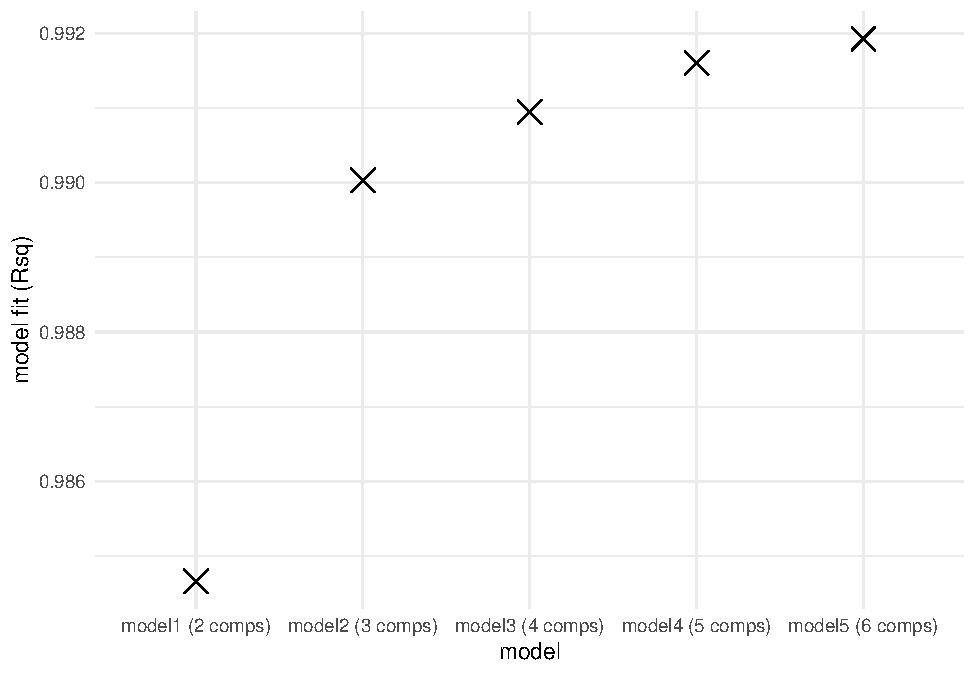
\includegraphics{220323_DWARF_sample_overview_and_EEM_files/figure-latex/First model attempt-1.pdf}
  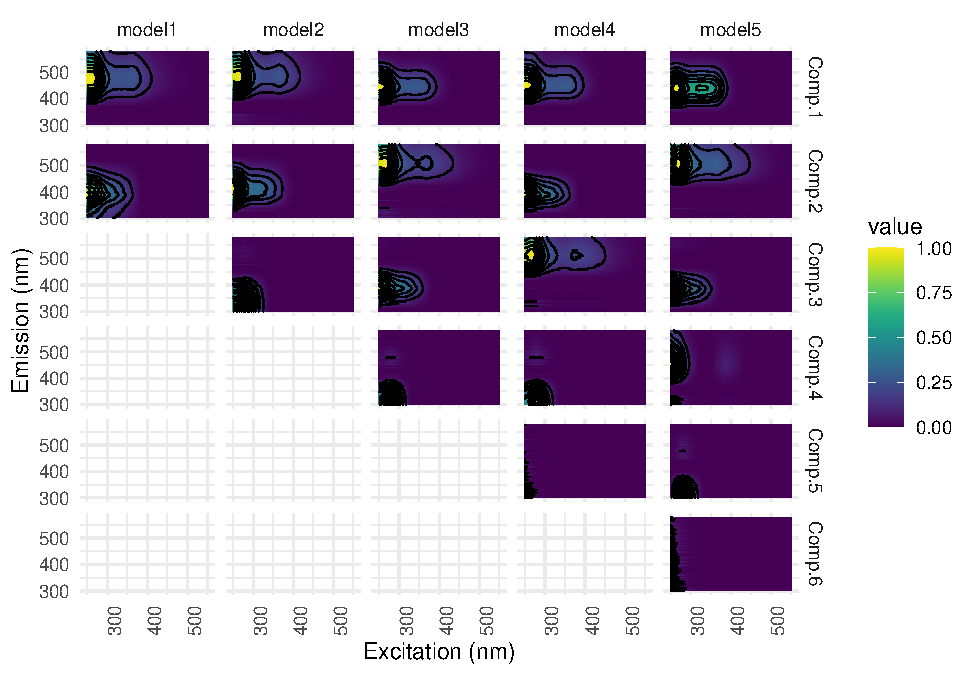
\includegraphics{220323_DWARF_sample_overview_and_EEM_files/figure-latex/First model attempt-2.pdf}
  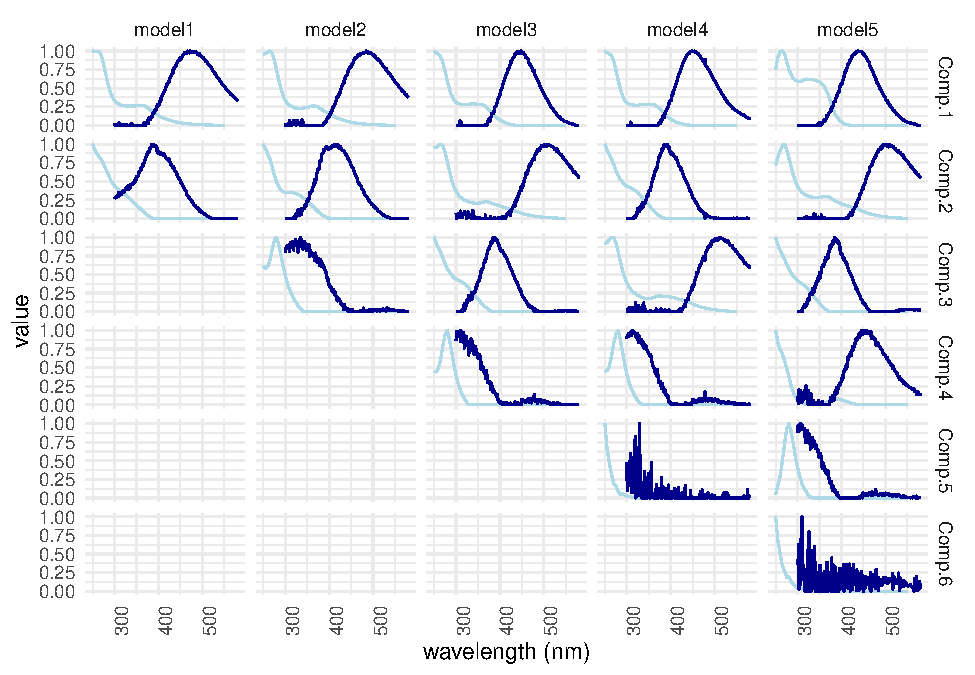
\includegraphics{220323_DWARF_sample_overview_and_EEM_files/figure-latex/First model attempt-3.pdf}
\end{itemize}

\begin{verbatim}
## [[1]]
\end{verbatim}

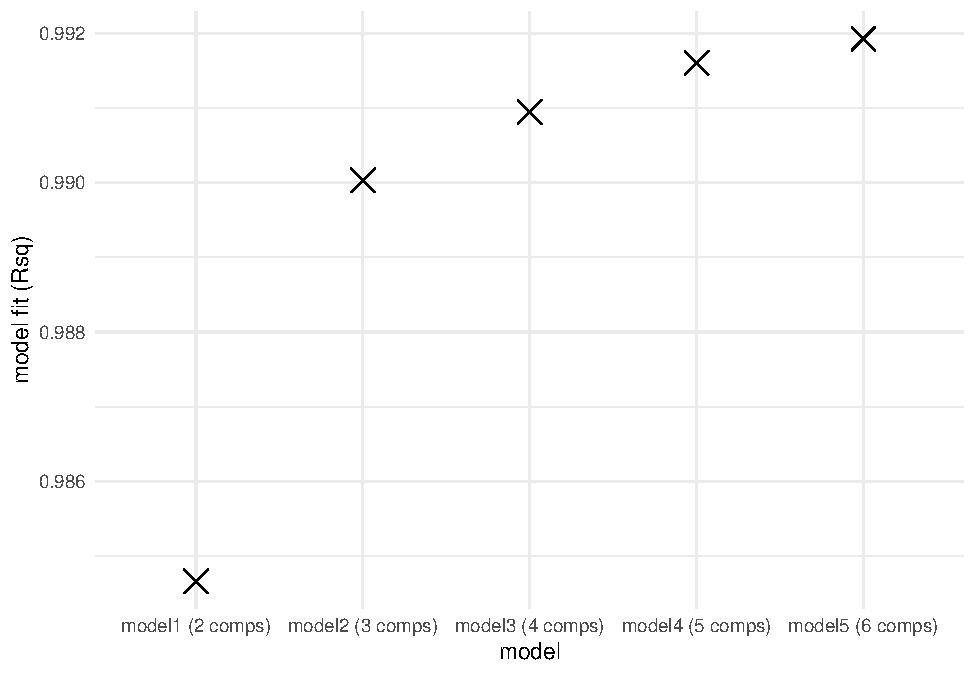
\includegraphics{220323_DWARF_sample_overview_and_EEM_files/figure-latex/First model attempt-4.pdf}

\begin{verbatim}
## 
## [[2]]
\end{verbatim}

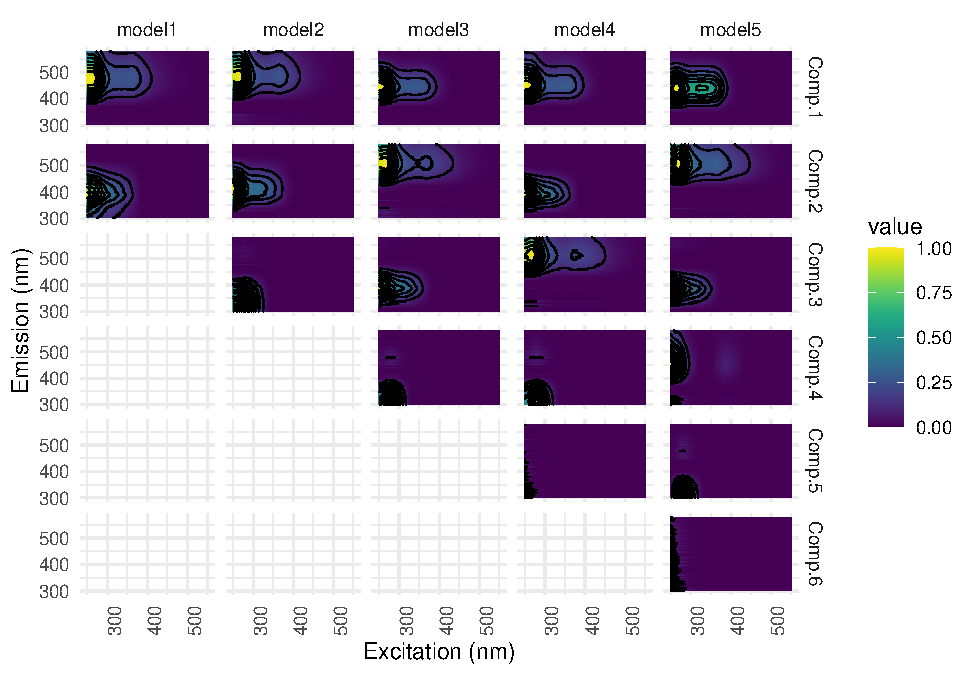
\includegraphics{220323_DWARF_sample_overview_and_EEM_files/figure-latex/First model attempt-5.pdf}

\begin{verbatim}
## 
## [[3]]
\end{verbatim}

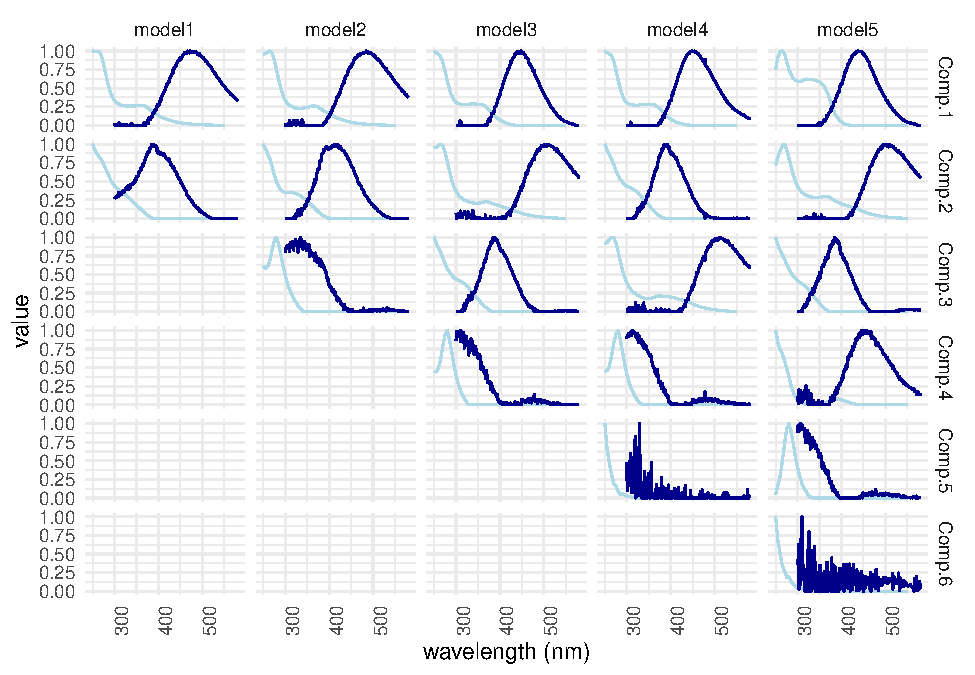
\includegraphics{220323_DWARF_sample_overview_and_EEM_files/figure-latex/First model attempt-6.pdf}

\includegraphics{220323_DWARF_sample_overview_and_EEM_files/figure-latex/First model checking: correlation between components-1.pdf}
\includegraphics{220323_DWARF_sample_overview_and_EEM_files/figure-latex/First model checking: correlation between components-2.pdf}

\hypertarget{step-4.-evaluate-extreme-sampleswavelengths}{%
\subsubsection{Step 4. Evaluate extreme
samples/wavelengths}\label{step-4.-evaluate-extreme-sampleswavelengths}}

\begin{itemize}
\tightlist
\item
  sometimes, extreme samples or emission/excitation wavelengths can be
  excluded from the sample set prior to making the PARAFAC model
\item
  dont appear to be any strong outliers (value from 0 to 1)
\item
  decides to keep all samples and wavelengths
  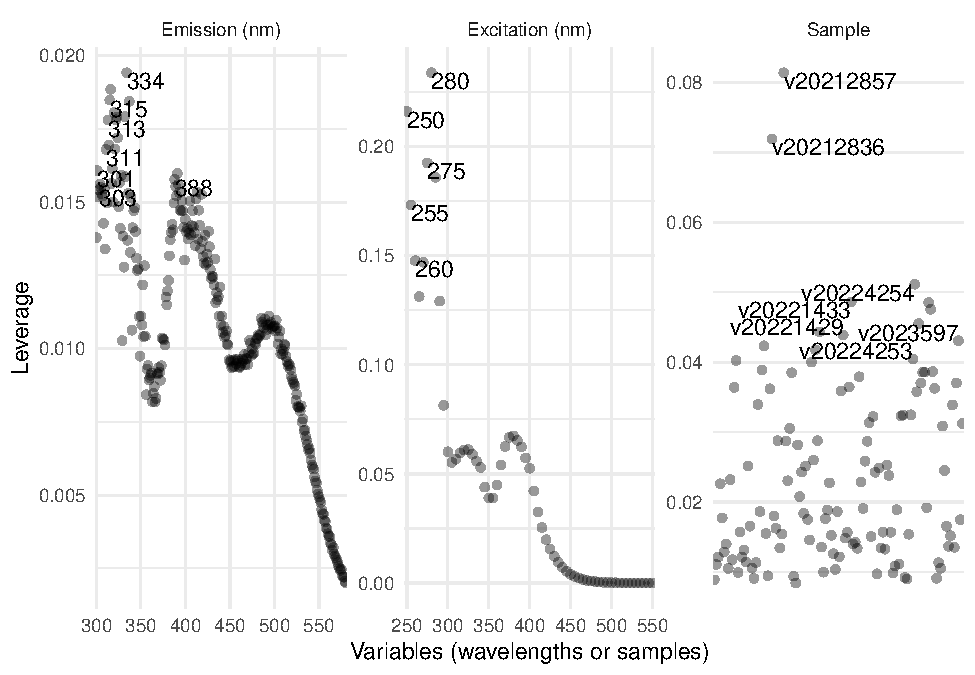
\includegraphics{220323_DWARF_sample_overview_and_EEM_files/figure-latex/Look for outliers in leverages-1.pdf}
\end{itemize}

\hypertarget{step-5.-re-run-parafac-model-with-increased-resolution}{%
\subsubsection{Step 5. Re-run PARAFAC model with increased
``resolution''}\label{step-5.-re-run-parafac-model-with-increased-resolution}}

\begin{itemize}
\tightlist
\item
  selects model no2 with 3 components
\end{itemize}

\hypertarget{step-6.-model-checking}{%
\subsubsection{Step 6. Model checking}\label{step-6.-model-checking}}

\begin{itemize}
\tightlist
\item
  several options are available, with their different advantagous and
  disadvantagous
\item
  some subjectivity is involved
\end{itemize}

\begin{verbatim}
## Calculated models:  50
## Converging models:  31
## Not converging Models, iteration limit reached:  0
## Not converging models, other reasons:  19
## Best SSE:  8151.815
## Summary of SSEs of converging models:
##    Min. 1st Qu.  Median    Mean 3rd Qu.    Max. 
##    8152    8152    8152    8152    8152    8152
\end{verbatim}

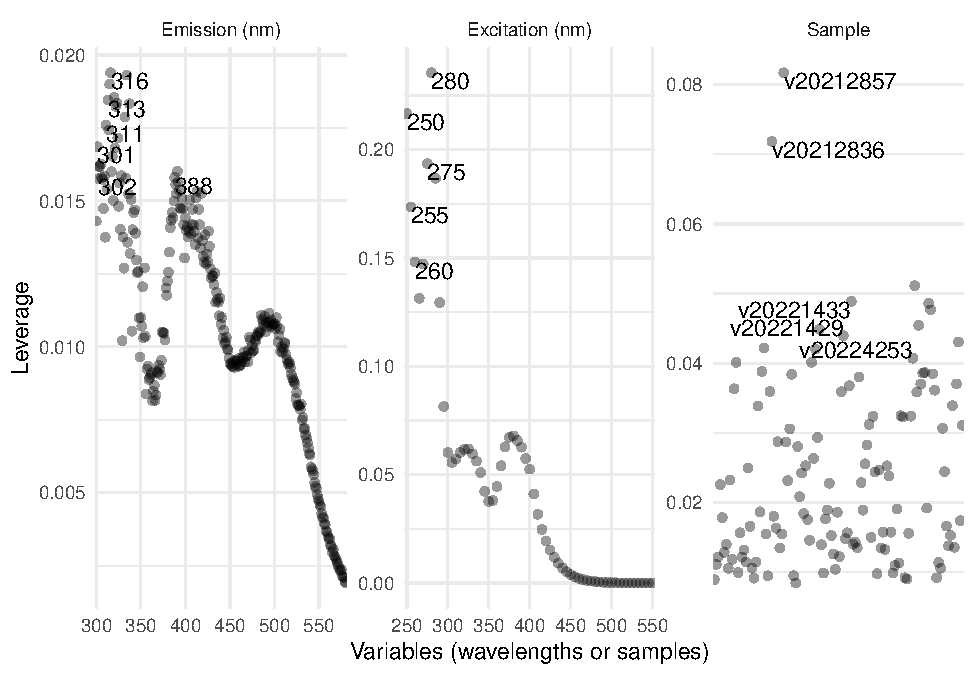
\includegraphics{220323_DWARF_sample_overview_and_EEM_files/figure-latex/Model checking-1.pdf}

\begin{verbatim}
## [[1]]
\end{verbatim}

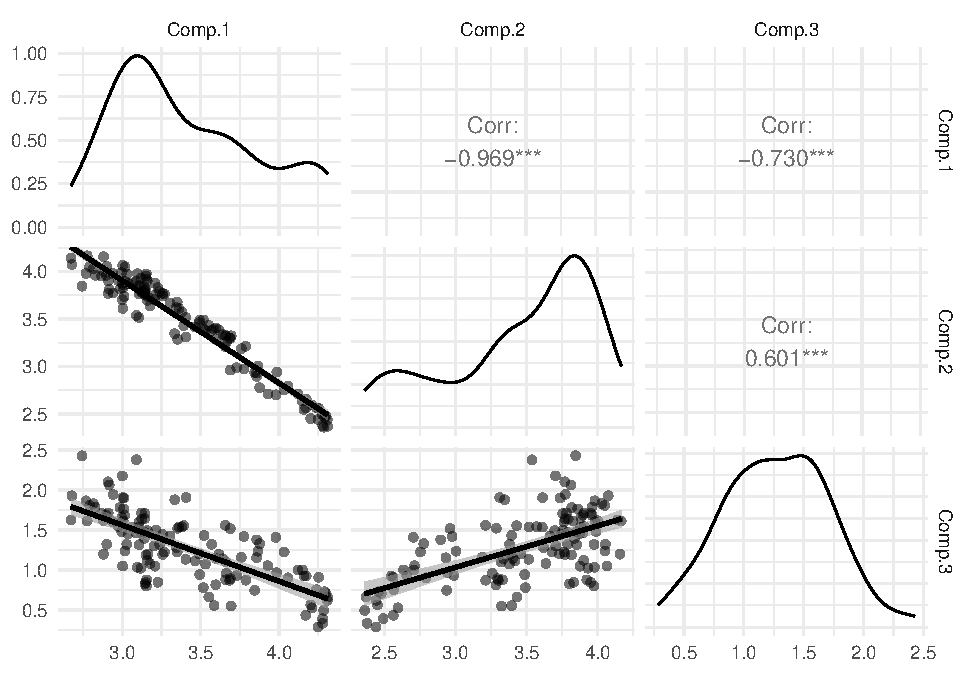
\includegraphics{220323_DWARF_sample_overview_and_EEM_files/figure-latex/Model checking-2.pdf}

\begin{verbatim}
## 
## [[2]]
\end{verbatim}

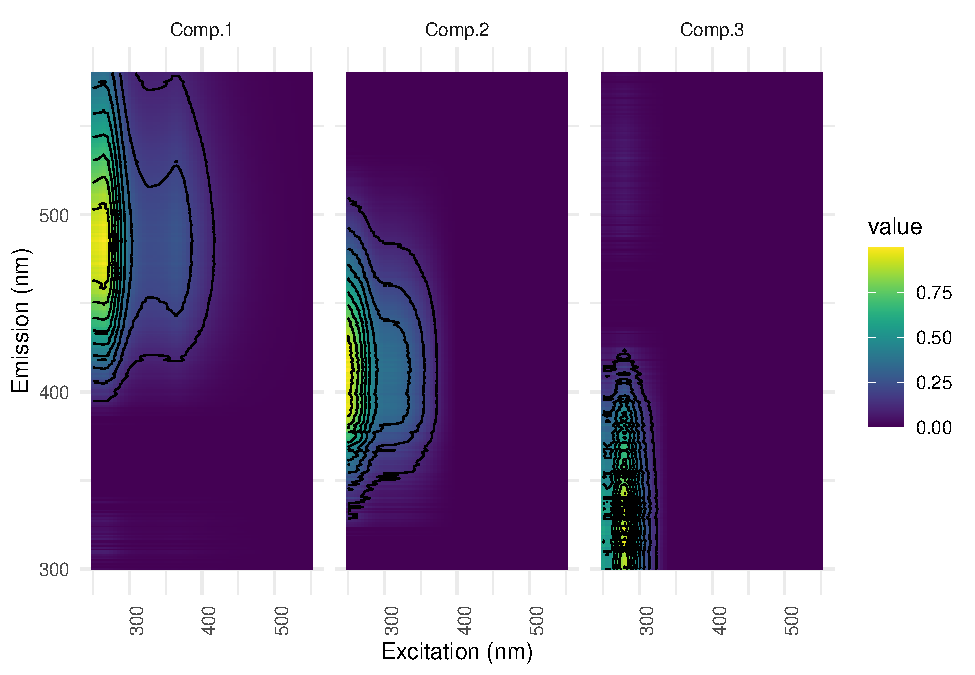
\includegraphics{220323_DWARF_sample_overview_and_EEM_files/figure-latex/Model checking-3.pdf}
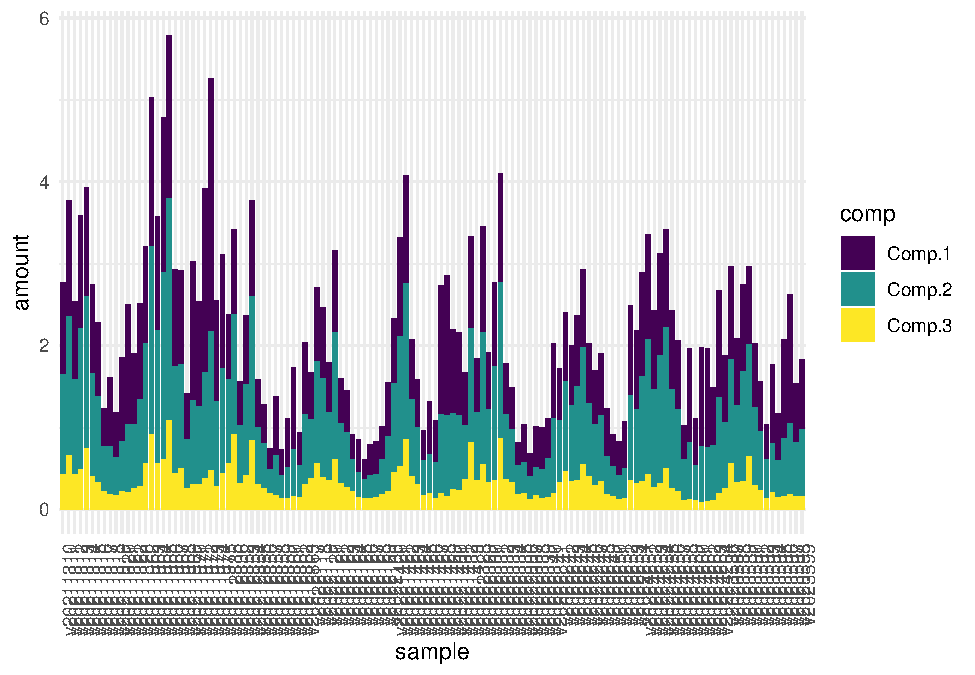
\includegraphics{220323_DWARF_sample_overview_and_EEM_files/figure-latex/Model checking-4.pdf}
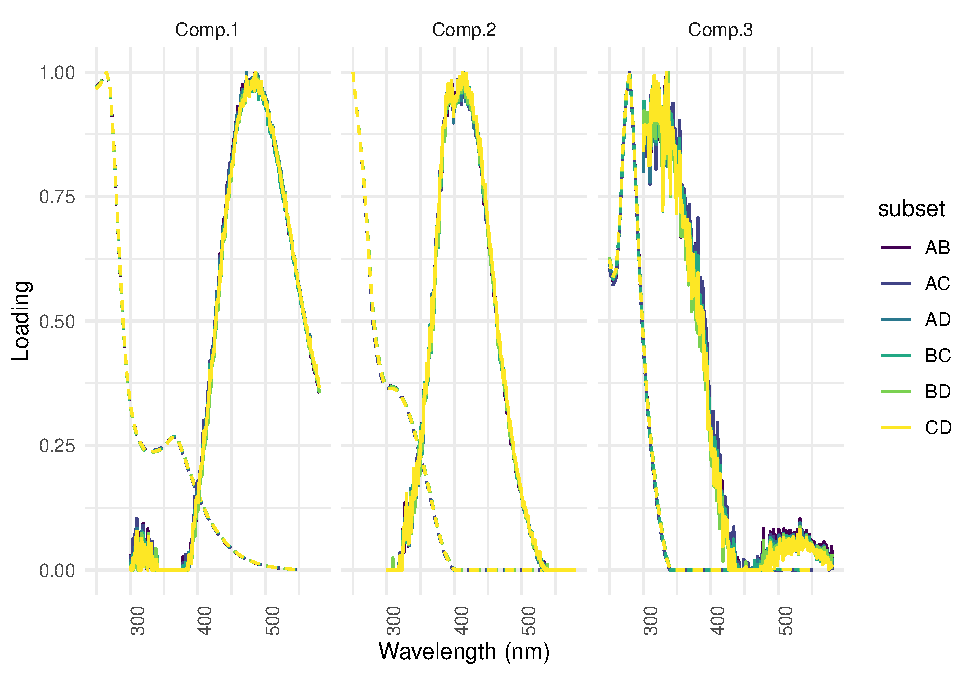
\includegraphics{220323_DWARF_sample_overview_and_EEM_files/figure-latex/Model checking-5.pdf}
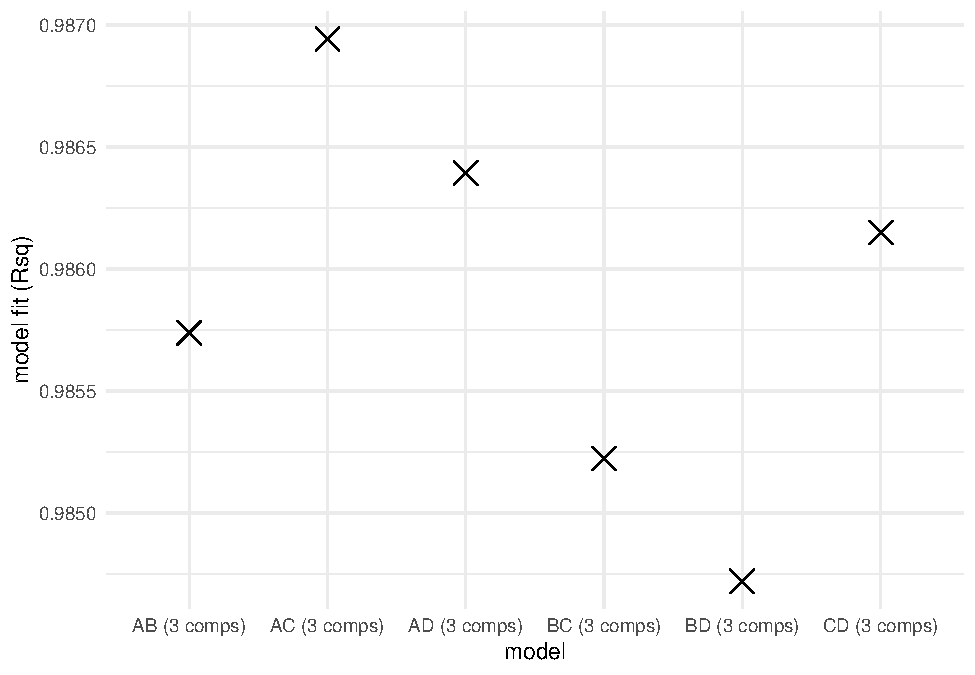
\includegraphics{220323_DWARF_sample_overview_and_EEM_files/figure-latex/Model checking-6.pdf}
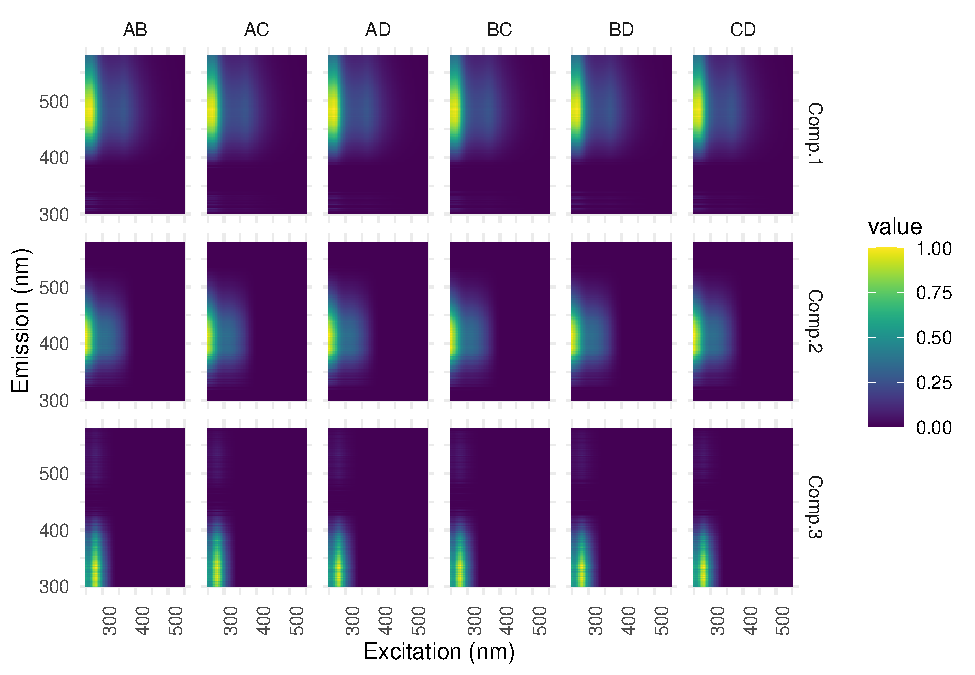
\includegraphics{220323_DWARF_sample_overview_and_EEM_files/figure-latex/Model checking-7.pdf}

\begin{verbatim}
## [[1]]
\end{verbatim}

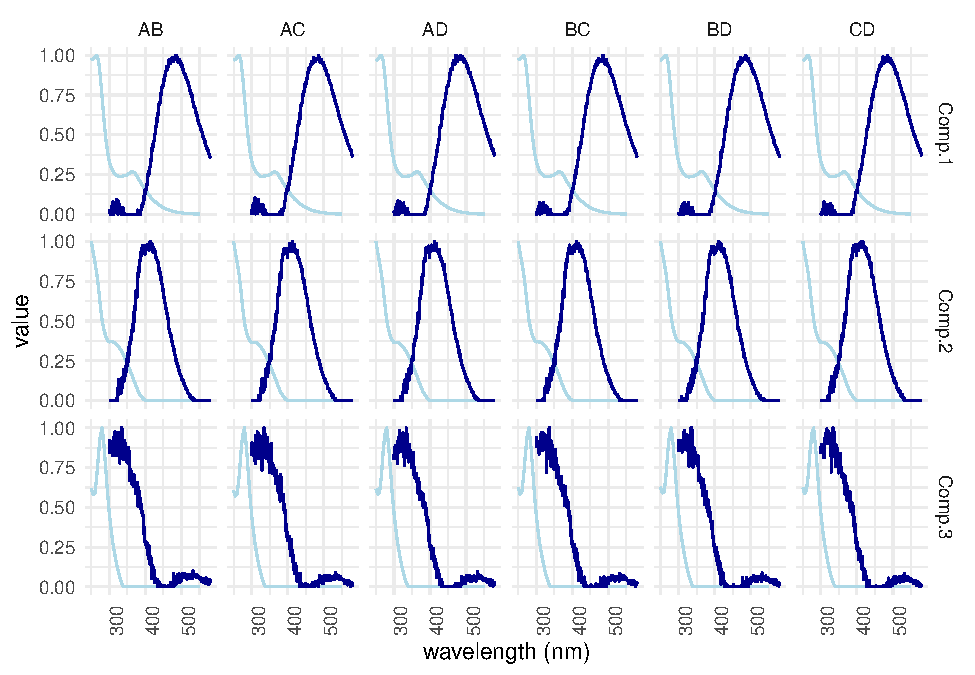
\includegraphics{220323_DWARF_sample_overview_and_EEM_files/figure-latex/Model checking-8.pdf}

\begin{verbatim}
## 
## [[2]]
\end{verbatim}

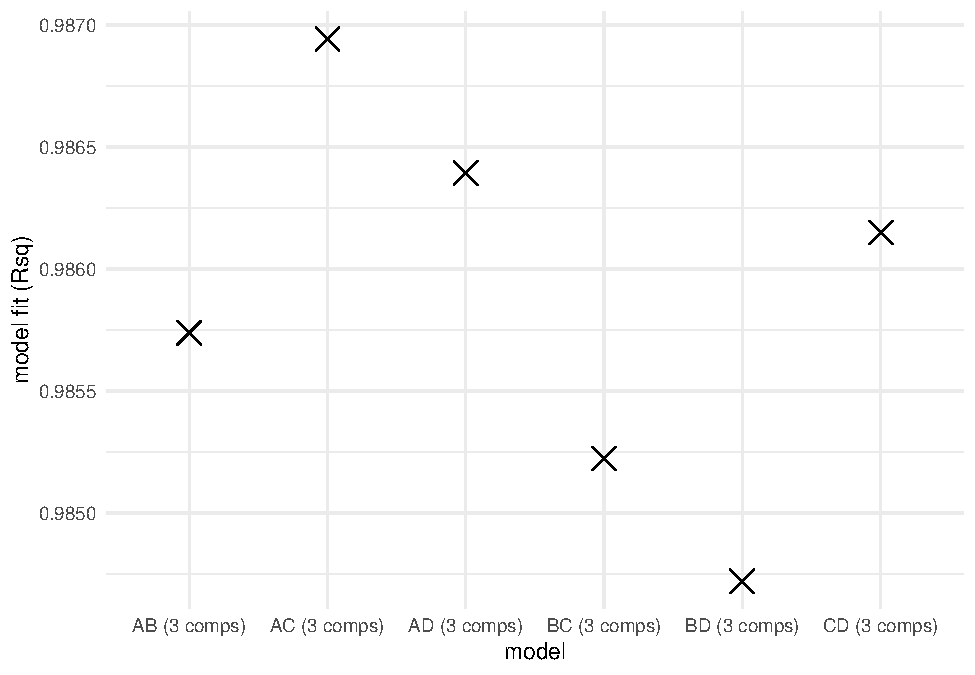
\includegraphics{220323_DWARF_sample_overview_and_EEM_files/figure-latex/Model checking-9.pdf}

\begin{verbatim}
## 
## [[3]]
\end{verbatim}

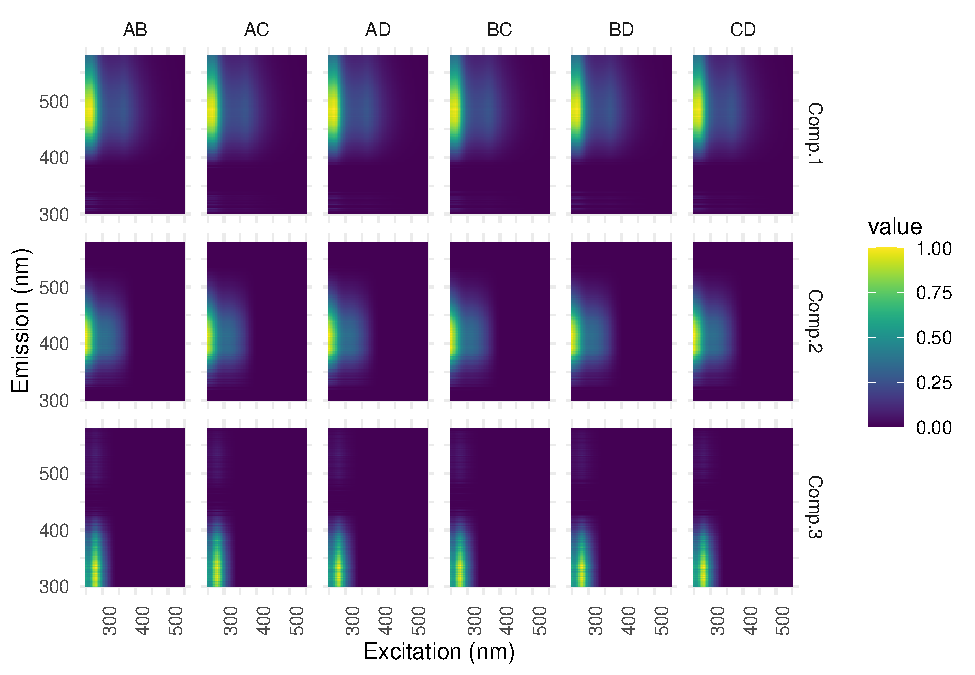
\includegraphics{220323_DWARF_sample_overview_and_EEM_files/figure-latex/Model checking-10.pdf}

\begin{verbatim}
##   component   comb    tcc_em    tcc_ex
## 1    Comp.1 ABvsCD 0.9999332 0.9997983
## 2    Comp.1 ACvsBD 0.9999962 0.9998863
## 3    Comp.1 ADvsBC 0.9999908 0.9998135
## 4    Comp.2 ABvsCD 0.9998731 0.9986536
## 5    Comp.2 ACvsBD 0.9999563 0.9998082
## 6    Comp.2 ADvsBC 0.9999197 0.9997846
## 7    Comp.3 ABvsCD 0.9999291 0.9974004
## 8    Comp.3 ACvsBD 0.9999505 0.9987646
## 9    Comp.3 ADvsBC 0.9997121 0.9988840
\end{verbatim}

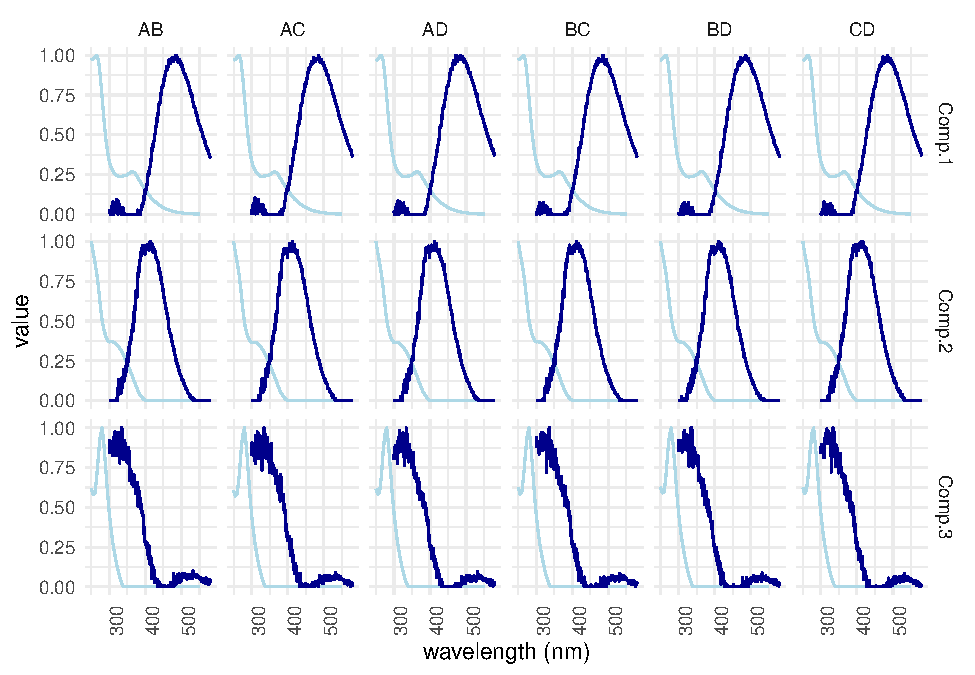
\includegraphics{220323_DWARF_sample_overview_and_EEM_files/figure-latex/Model checking-11.pdf}

\begin{verbatim}
##   component   comb    tcc_em    tcc_ex
## 1    Comp.1 ABvsCD 0.9998564 0.9996464
## 2    Comp.1 ACvsBD 0.9998620 0.9983815
## 3    Comp.1 ADvsBC 0.9999670 0.9997049
## 4    Comp.2 ABvsCD 0.9990952 0.9988607
## 5    Comp.2 ACvsBD 0.9998315 0.9982346
## 6    Comp.2 ADvsBC 0.9997609 0.9996929
## 7    Comp.3 ABvsCD 0.9995324 0.9833497
## 8    Comp.3 ACvsBD 0.9998618 0.9981210
## 9    Comp.3 ADvsBC 0.9993963 0.9979928
\end{verbatim}

\begin{verbatim}
## [1] 0.26436032 0.14581703 0.02835108
\end{verbatim}

\hypertarget{step-6.-results-created-model-is-exported-to-openfluor-to-compare-with-other-studies-and-identify-the-components}{%
\subsubsection{Step 6. RESULTS: Created model is exported to OpenFluor
to compare with other studies and identify the
components}\label{step-6.-results-created-model-is-exported-to-openfluor-to-compare-with-other-studies-and-identify-the-components}}

From OpenFluor the following can be linked to the model components: *
C1: Humic-material, larger-sized, characteristic of soil, sediment and
freshwater environments, recalcitrant soil or plant material, highly
resistant to microbial degradation but suspictible to photodecay
(\url{https://doi.org/10.1016/j.geoderma.2017.06.029}), similar to
soil-fulvic material (10.1080/00785236.2003.10409512), larger sized
humics from cultivated soils (10.1016/j.jaridenv.2019.04.013),
Terrestrial humic-like fluorescence in high nutrient and wastewater
impacted environments (10.1021/es103015e), Humic-like Terrestrial
delivered OM (10.1016/j.watres.2014.01.053) * C2: Humic-material,
mid-sized, characteristic of soil, sediment and freshwater environments,
recalcitrant soil or plant material, highly resistant to microbial
degradation but susceptible to photodecay
(\url{https://doi.org/10.1016/j.geoderma.2017.06.029}), terrestrial
humic-like (e.g.~Painter et al.2018); microbially- or photo-chemically
altered organic matter (Yamashita et al.~2013)
(10.1088/1748-9326/abac36) * C3: protein-like material
(tryptophane/tyrosine), often linked to anthropogenic distrubances
(10.1890/12-0825.1), protein-like (10.1890/12-0825.1), biological- and
fresh production (10.1016/j.marchem.2019.103720)

\begin{longtable}[]{@{}lcr@{}}
\toprule
Component & Ex. max (nm) & Em. max (nm) \\
\midrule
\endhead
C1 & 265/365 & 485 \\
C2 & 250/310 & 412 \\
C3 & 280 & 321 \\
\bottomrule
\end{longtable}

\end{document}
